%!TEX root = ../../super_main.tex

\section{Extreme Programming}
\label{sec:extreme_programming}

In this project we have chosen to use some of the aspects from the Extreme Programming (XP) method, which is a type of agile software development method, that has a high amount of focus on customer satisfaction, developer productivity/welfare and high product quality \parencite{xp}. The method focuses on delivering partial products to the customers as they need them, instead of just a complete product far in the future. In XP this is normally achieved by use of several core practices, such as: on-site customer, test driven development, pair programming, planning poker, continuous integration and delivery and daily meetings. XP emphasizes the value of \emph{simplicity}, \emph{communication}, \emph{feedback}, \emph{respect}, and \emph{courage}. 

\begin{itemize}
	\item \emph{Simplicity} is about taking the simplest path to delivering a minimum viable product without compromising quality. 
	\item \emph{Communication} between every member of the team, including the on site customers, is essential to deliver a product that everybody is proud of. 
	\item \emph{Feedback} should be taken seriously, and demonstrations should be done early in the process and frequently.
	\item \emph{Respect} between the team members, the customers, and management is important.
	\item \emph{Courage} allows the team to take on new challenges without the fear of failing, because nobody works alone. The developers should have the courage to tell the truth about progress and estimates. 
\end{itemize}

The following sections will describe some of the basic concepts from the XP method that we have chosen to use, how we have implemented them, and some of the conflicts there are between our project and the method.

\subsection{Iterations}
\label{sub:iterations}
Extreme Programming encourages rather short iterations in comparison to other agile development methods. The iterations are of constant length and should be between one to three weeks in length. Because of their constant length they can be used to track the progression and the velocity of a project by evaluating the amount of work done in the end of an iteration compared to the estimates given to the tasks in the given iteration. 
\\\\
In our project we have chosen to use iterations of two weeks (calendar time) in length. Each of these will end with a review of what we have managed to accomplish in the given iteration. One of the issues with using calendar time to schedule our iterations is the fact that we are students, meaning that we have to follow the courses on the semester as well. This makes the amount of time we have available vary between the different iterations, making it more difficult to estimate how much we can handle in each iteration. To try to alleviate this issue we calculate the amount of time we have in a given iteration and take that into consideration when planning it. 

\subsection{Releases}
XP encourages frequent and small releases to the customers. Each iteration ends with a deliverable in XP and these deliverables can be evaluated by the customer, who then can decide if it should be taken into production. The idea behind frequent releases is that the earlier the functionality is used by the customers, the sooner any potential bugs can be found and fixed by the developers. Furthermore, it allows the customers and the team to evaluate if the project is on the right track.
\\\\
We have chosen to make a release every second XP iteration, meaning that we will make a release every four weeks. For each of the releases we will make a major product release, but we will also build a minor product release for iterations that do not end in an XP release, if the product is accepted by the customer at the given time. All releases are pushed to our \href{https://github.com/Shaderex/SW8-Android/releases}{GitHub Page}\footnote{\url{https://github.com/Shaderex/SW8-Android/releases}} and can also be found on the CD in \todo{Add reference to CD appendix}. The deliverables for each iteration we have completed are described in \todo{Ref til appendix med Deliverables}. 

\todo[inline]{Beskriv hvad vi gør for at bestemme om produktet er klar til produktion}

\subsection{Taskboard and User Stories}
\label{sub:taskboard_and_user_stories}
In XP a release plan is created for each release, during a release planning meeting. The release plan is typically represented on a taskboard by the use of user story cards and task cards. An example of such a taskboard can be seen in \figref{fig:taskboard}.

\begin{figure}[!htbp]
    \centering
    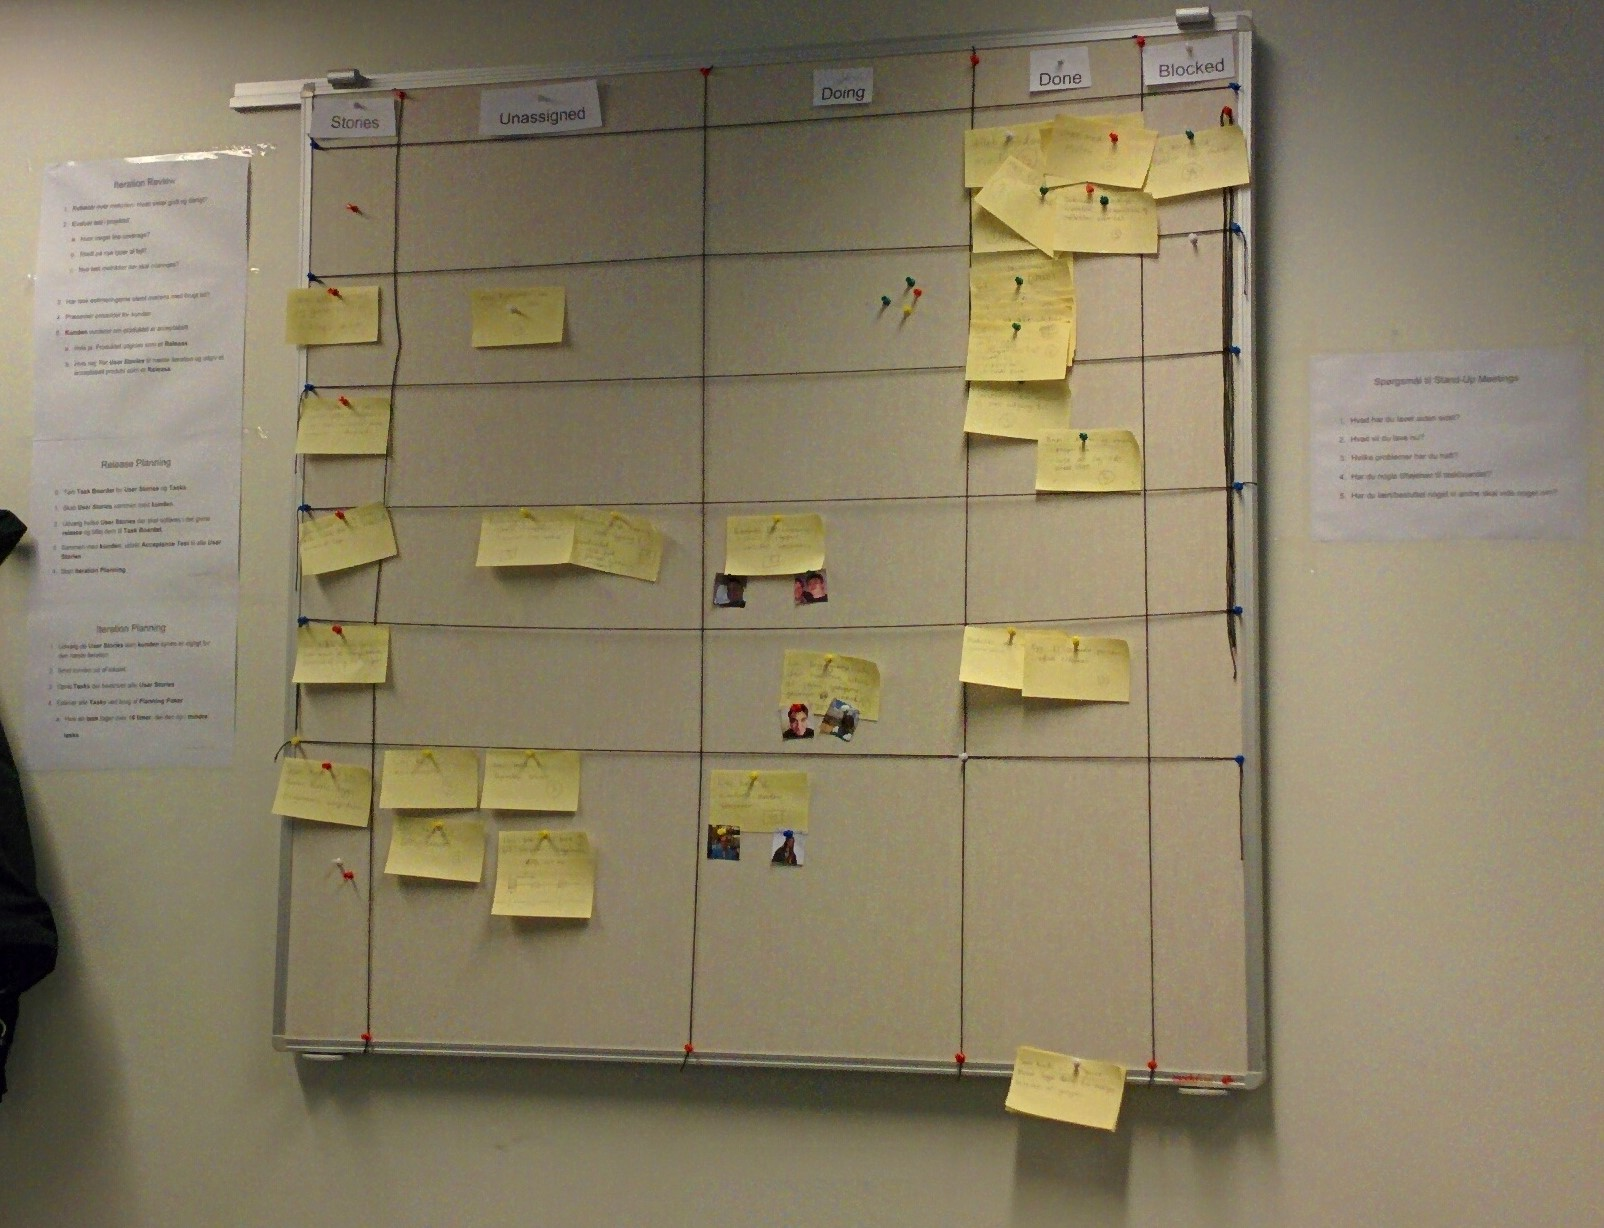
\includegraphics[width=0.7\textwidth]{method/taskboard.jpg}
    \caption{A picture of our taskboard.}
    \label{fig:taskboard}
\end{figure}

The user story cards are made in collaboration with the customer during release planning.  A subset of all the stories will then be selected to be completed in the given iteration, and acceptance tests will be made for these stories. An acceptance test is a specific test that is conducted in order to determine whether the specification or contract is met. And example of a user story and corresponding acceptance test can be seen in \tabref{tab:user_story_acceptance_test_example}. The rest of the user stories and acceptance tests can be found in \appref{app:user_stories_and_acceptance_test}.

\begin{table}[!htbp]
    \begin{tabular}{| m{0.45\textwidth} | m{0.45\textwidth} |}
        \hline
        \textbf{User Story} & \textbf{Acceptance Test} \\ \hline
        As a customer, I would like to get answers from questionnaires generated by me from participants & 
        \begin{itemize}[noitemsep,parsep=0pt,partopsep=0pt]
        \item When a customer can come up with a questionnaire, get it into the system without writing code, and have it answered by a participant.
        \item The questions must occur in sequence and it should only be possible to answer yes or no.
     \end{itemize} \\ \hline
    \end{tabular}
    \caption{Example of a user story and corresponding acceptance test from our first iteration.}
    \label{tab:user_story_acceptance_test_example}
\end{table}
\FloatBarrier

We have chosen attempt to follow the standard XP release plan concept by playing various roles from XP, because they are such a central aspect of the method. For this reason during the iteration review and planning meetings we assign each team member roles, such as customer, tester, developer, and user, which they must role-play. This role playing makes it easier for us, as a team, to prioritize user story cards because one team member only has to consider one mindset during these meetings. This approach might be challenging because it can be difficult to apply a different mindset than what we are used to. This means that one team member is assigned to act as the customer during the entire review/planning meeting. As mentioned previously, another central aspect of the development is to have a representative for the customer on-site. However, this project is a student project without a paying customer or user, and we have therefore dediced to include role-play to compensate for this. 

\todo[inline]{Måske tilføje argument omkring innovation og at der ikke behøver at være en dedikeret customer - Måske tilføje noget med at role play så er baseret på et vision?}

\subsection{Knowledge Sharing}
\label{sub:knowledge_sharing}
Knowledge sharing is encouraged in XP by using different practices such as daily stand up meetings. Daily stand up meetings are short meetings where the group members share thoughts about their current progress, hardships, and successes. This allows for brief insight in the collective progress of the group. Another core practice is pair programming, where two programmers sit at the same PC and develop together. Even though the main purpose of pair programming is to increase code quality it also allows for knowledge sharing between the programmers. 
\\\\ 
For us, knowledge sharing is important, since all members of the group should have insight in the product and the written report. We have therefore chosen to use daily stand ups and pair programming / writing in our process. We expect that these practices will increase the feeling of collective ownership over the project, provide a steady pace during development, and increase the quality of the project. 

\subsection{Test Driven Development}
\label{sub:test_driven_development}
Extreme Programming emphasizes that test driven development is the only development method that ensures that the developed program works as intended and is tested without using any shortcuts (i.e. the developer writes test-to-pass instead of test-to-fail). In previous semesters we have been lacking a structured approach to testing and evaluating during the development. Tests and evaluations have therefore previously been executed in ad-hoc fashions, which has not been as useful for us as we could have hoped. In an agile development method, we hope that a test-driven approach will help us solve this problem and achieve a more structured approach to enforce testing and increase code quality.
\\\\
We have not been working with XP or general acceptance testing in previous semester projects, and we therefore cannot judge the quality of the acceptance tests we will create for our user stories.

\subsection{Documentation}
A major part of the XP method is to maintain focus on development and not documentation, and it is only considered in XP if it gives the customer value. This is a very counter-intuitive approach in a student setting, because we have a requirement for the project that states necessary documentation. 
\\\\
Due to the fact that XP does not not have any built in practices or techniques to produce a technical student report during development, we have to adapt our development method to include the production of such a report. We attempt to do this by integrating development 

\todo[inline]{Skriv det her færdigt!}









